\documentclass[10pt,a4paper]{scrartcl}
\usepackage[utf8]{inputenc}
\usepackage[english]{babel}
\usepackage{color}
\usepackage[pdftex]{graphicx}
\usepackage{natbib}
\usepackage{hyperref}

\title{Study on the Club of Rome's World3 Model}
\subtitle{Project Introduction to Computational Science 2014\\
University of Amsterdam}
\author{Marc Went, student number 10905847\\Ferry Avis, student number 10904581}

\begin{document}

\maketitle

\section*{Introduction}

This report describes the modelling and simulation project for the course Introduction to Computational Science of the college year 2014-2015 at the University of Amsterdam. The aim of the project is to perform a science project, which will be supported by a simulation study.

For the simulation study, we will investigate the Club of Rome's World3 model, which models interactions between industrial growth, population, food production and pollution. 

\section*{Background of the model and its use}

In 1968, a group of people from politics, business and science came together to \emph{"discuss the dilemma of prevailing short-term thinking in international affairs and, in particular, the concerns regarding unlimited resource consumption in an increasingly interdependent world"}. This group was named \emph{The Club of Rome}, after the location of the meeting. The first and subsequent meetings resulted in the book `\emph{Limits to Growth}', published in 1972. In the book it was predicted that economic growth could not continue indefinitely, mainly because of the limited availability of natural resources and emissions. Somewhere in the twenty-first century, the growth would end in a uncontrolled decline in population and human welfare.

The underlying model used in the study is the World3 model. It was the first model that used computer simulation to model the interactions of five sub models, which represent capital, natural resources, agriculture, population and pollution, on a global scale.

It has to be noted that World3 model is far from perfect and was merely a first step in modelling the global world. The authors point out the use of inadequate data, the usage of quantifications of factors for which the influence is not fully clear, such as pollution, and unknown development of technology in the future. Also, natural resources are seen as one identity, while in reality substitutions of depleted natural resources are possible. Increasing prices because of scarcity and the stabilising working of the law of supply and demand are missing in the World3 model; very different from assumptions economists often make in their models.

Despite its flaws, the World3 model is suitable enough to illustrate the validity of the Club of Rome's hypotheses. The model is an example that it is not necessary to have a perfect model to give an clear insight in problems. The model does not give a prediction, but is sketching alternative scenario's for humanity. For taking appropriate measures to prevent a scenario becoming true, the model and its validity need to be studied and improved extensively. The World3 model shows what possibly can go wrong. \cite{vermeulen1976parameter} conclude that, while in \emph{Limits to Growth} very severe measures are suggested for every subsector in the world model in order to avoid the catastrophic population collapse of the standard run, that by combining three changes of 10\% each in the parameters ICOR, FIOAC, ALIC, the collapse of population can also be avoided. They speculate that the real world has so many variables and is so flexible that the correct small pressures on the correct parameters could cause desirable outcomes for the world's evolution.

Despite the large amount of publicity Limits to Growth has received at publication, concerned governments continued to go everything they could to stimulate economic growth and no start was made for a transition to a sustainable growth. This was mainly to reduce unemployment. \cite{voorbijdegrenzen} believes that the main contribution of the report is that it led to a continued interest in future of humanity and the start of many discussions.

The difficulty of the problem is that no single country is responsible on its own or able to take appropriate actions. Measures on a world wide scale are necessary, which are very difficult to coordinate. The history of the ozone hole and acid rain shows that global coordination is not impossible. In this report, we will not elaborate on the subject of international cooperation.

\subsubsection*{Critics on the World3 model and Limits to Growth}

The report and the model have received many critics. However, changing the model does not change the conclusion: unlimited growth cannot continue. Some people argued that the equation $y(t) = ae^{rt}$ is also sufficient to show that sustainable growth cannot continue.

Economists often address that the used assumptions in the models are very different from the axiom's economists often use. Also, the tone of the report is pessimistic. The Club of Rome was wrongfully called the zero growth movement, although the conclusion of the report does not to deny this qualification. In the report there is a dedicated chapter about the conditions to obtain sustainable growth and what growth in a global equilibrium means. Within these conditions, company's can rise and fall, local population can grow and decline. Technological developments can improve the average standard of living.

\section*{Standard run of the model}

Figure \ref{standard-run} shows the behaviour of the standard model, i.e. of the model when no changes to the parameters are made.

\begin{figure}
\centering
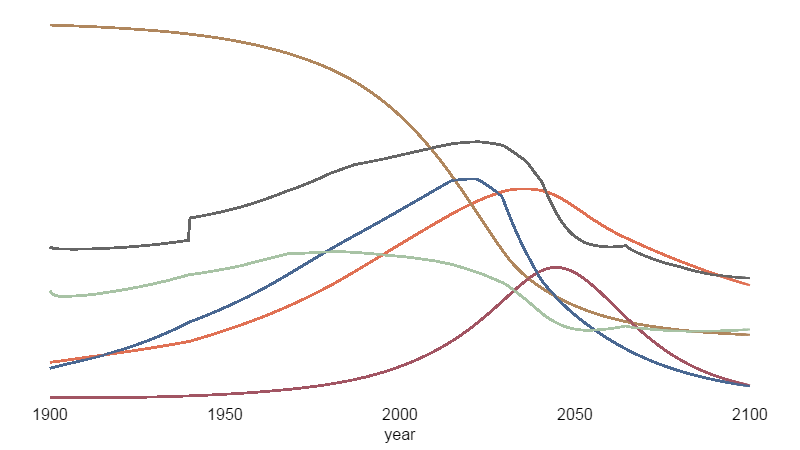
\includegraphics[width=\textwidth]{./plaatjes/standard-run.png}
\caption{Behaviour of the model in the standard run}
\label{standard-run}
\end{figure}

Note that the scale on the y-axis is missing. The model does not give predictions, but a direction. The numbers are very likely to be inaccurate and are thus not of great importance.

The model shown in Figure 1 shows that around 2040 society will collapse. This happens shortly after the industrial output drops. This manifestation of these catastrophes is an indication that not only the resources are depleted but also the pollution of this world is rising to a record high.

The rising pollution also has a big effect on the life expectancy of the population. Figure 1 shows a correlation around 2045, where pollution is at the largest peak and the life expectancy drops rapidly. Since the turn of a rising life expectancy to a dropping one, the population growth has stagnated, which results in a decay of the human population.

\section*{Research questions}

A full analysis of the parameters of model, the influences of the submodels and making simplifications is enough to write a PhD thesis: see \cite{thissen1978investigations}. However, we would like to study small parts of the model. Based on our own interests and the discussion of the model in \cite{thissen1978investigations} and \cite{vermeulen1976parameter}, we ask the following questions:

\begin{itemize}
	\item What is the influence of the size of the population on the use of natural resources?
	\item Can the collapse of population indeed be ICOR and FIOAC increased by 10\% and ALIC decreased by 10\%.
	\item What is the influence of the amount of available natural resources on the other submodels?
	\item Do the conditions in the Limits to Growth to obtain sustainable growth indeed lead to a sustainable equilibrium?
\end{itemize}

Additionally, we will investigate behaviour of the model we find remarkable while varying parameters.

\section*{Implementation of the model}

The World3 model is an example of a model in the System dynamics formulation, which is based on feedback loops. Figure \ref{world3} An overview of the model and the interactions between the submodels. We included this figure to give an impression of the size of the model, not for details.

\begin{figure}
\centering
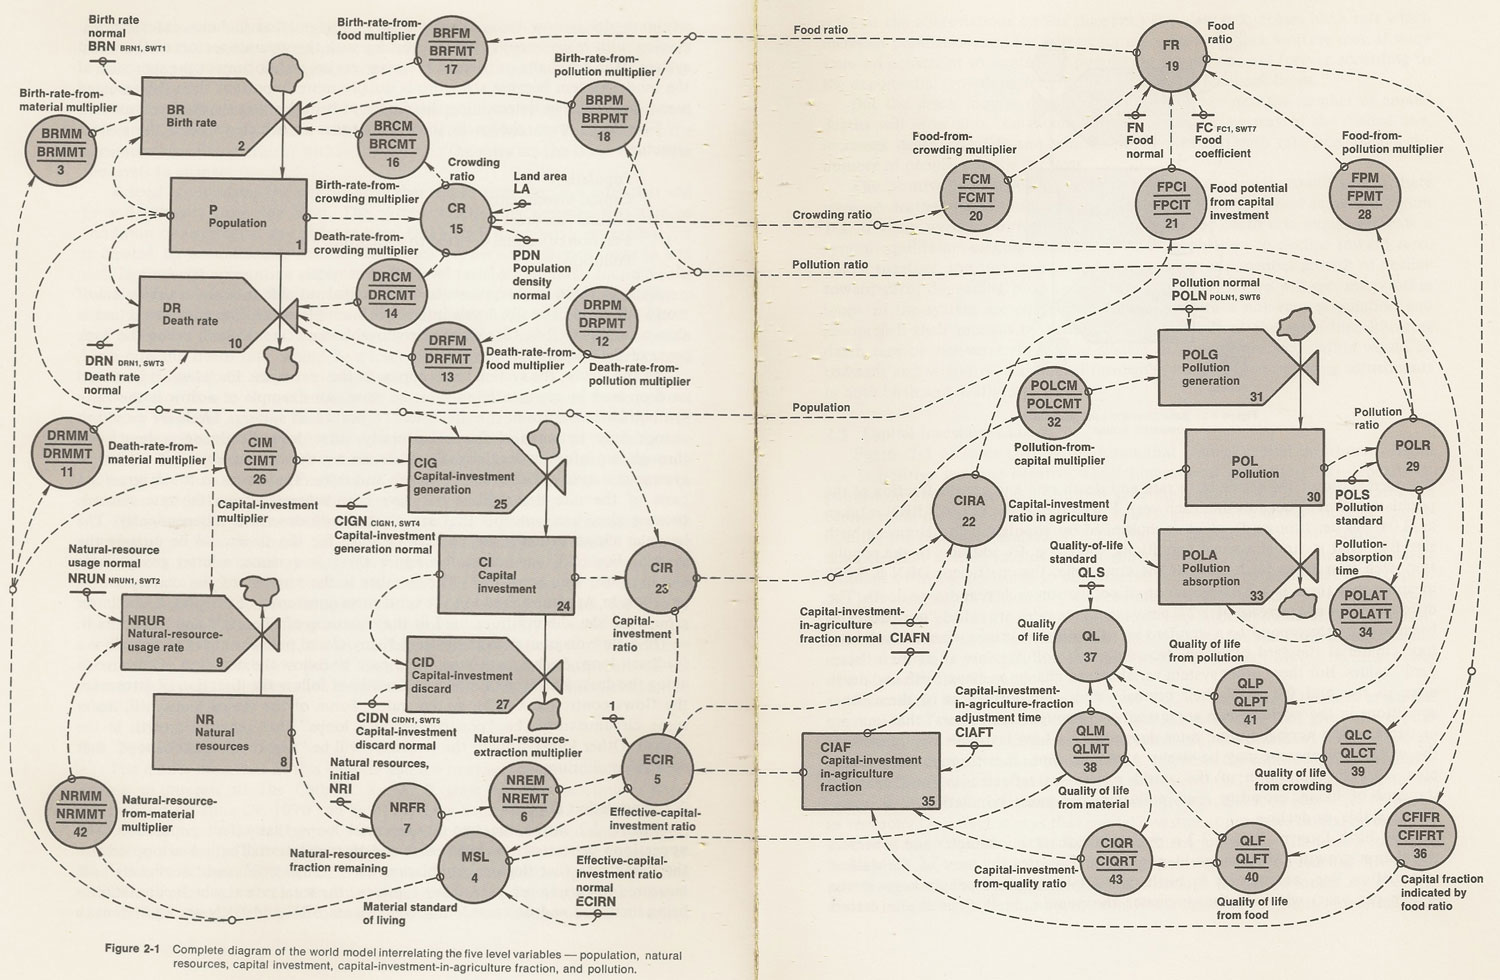
\includegraphics[width=\textwidth]{./plaatjes/model.jpg}
\caption{Diagram of the world model from cite{forresterworld}}
\label{world3}
\end{figure}

The complete model consists of more than 150 differential equations. The original model is formulated in a special language called DYNAMO. The model has since then be ported by the original authors to STELLA and extended to include human welfare and footprint indicators. Many others have created ports of the DYNAMO formulation to other languages, such as Java (\url{http://www.world3simulator.org/}), Vensim (\url{http://models.metasd.com/tag/world3/}) and JavaScript (\url{http://bit-player.org/extras/limits/}).

As we wanted to learn how to implement such large model, we tried to implement the World3 in the formulation as described in \cite{thissen1978investigations} in Python. In Thissen's formulation, the capital and resource subsectors are merged. However, we did not succeed. First, we will discuss our problems and use one of the ported versions of others for an analysis of the model.

First of all we implemented a simplified capital model. \cite{thissen1978investigations} suggested that differences neither population, agriculture or pollution has any major effect on the capital. This simplified model therefore uses constants for input of these submodels as an alternative. This model shows a proper approximation of the population prediction with the original World3 model.

As we thought this model was too easy we started to replace this simplified capital model with the extended capital model. This model relies on the three other submodels – population, agriculture and pollution. These were also implemented.

\subsection*{Simplified resource and capital model}

We were able to implement the simplified resource and capital model from \cite{thissen1978investigations}.

\textcolor{red}{Picture of the standard run in the simplified model and differences with the standard standard run}

\subsection*{Implementation of Will Thissen's full formulation}

Our implementation of Will Thissen's model does not give correct results.

A particular problem we encountered at the implementation is the use of a function from DYNAMO called DELAY3. This function represents a third-order linear delay. Although this function is implemented in and documented for Vensim, we were not able to find an explanation we could understand. Therefore it cannot be determined why the model does not behave the way it should.

To come up with a working model, we probably need to understand and implement the original model formulation from \cite{forresterworld} instead of the formulation from \cite{thissen1978investigations}. DYNAMO is an old language, with the special feature that equations can be written down in any order. The compiler does reorder the equations automatically. We expect this to be very challenging to implement this in a sequential language as Python.  After implementing the model in the sequential way, we discovered that the author of the JavaScript port also failed at implementing the model sequentially (\cite{blogpost}). Eventually, he mimicked the automatic ordering of equations of the DYNAMO compiler in JavaScript, but we are not fluent in JavaScript enough to study his approach.

Unfortunately, we do not have access to the newer STELLA formulation.

\subsubsection*{Steps taken to find the mistake}

The model was of course checked for typing errors. We corrected some, but this didn't lead to a working model.

\section*{Results and analysis}

Illustration of the delay of collapse when natural resources are increased. One of the examples of the use of incorrect data was the amount of available natural resources. New techniques have made it, for example, possible to extract oil deeper from the earth. However, as we will see, this will only delay the point.

\section*{The Club of Rome today}

Today, the Club of Rome still exists. The focus in its early years was on the nature of the global problems and on new pathways for world development. Currently, the Club of Rome defines and communicates the elements of a new economy, which produces real wealth and well-being, without degrading natural resources and and with providing meaningful jobs and sufficient income for all people.

Believe in advance of technique that we can solve problems in future

\section*{Conclusion}

The World3 model and Limits to Growth discusses interesting and urgent problems. A full analysis of the model has proven to be enough work for a PhD thesis. The model than this assignment 

\bibliographystyle{abbrvnat}
\nocite{*}
\bibliography{bibliografie}

\end{document}